\documentclass{beamer}
\usepackage[czech]{babel}
\usepackage[utf8]{inputenc}
\usepackage{minted}
\usetheme{Madrid}
\hypersetup{unicode=true}

\title{Lineární seznam}
\author{Martin Zmitko}
\institute[VUT FIT]{Vysoké učení technické v Brně\\
Fakulta informačních technologií}
\date{\today}

\begin{document}

\frame{\titlepage}

\begin{frame}
\frametitle{Obsah}
\tableofcontents
\end{frame}

\section{Co je to lineární seznam?}
\begin{frame}
\frametitle{Co je to lineární seznam?}
\begin{itemize}
    \item Je to seznam prvků, které na sebe vzájemně ukazují
    \item Každá struktura obsahuje samotné data a ukazatel na další prvek
    \item Lineární seznam je dynamická struktura, jeho velikost se tedy může měnit a prvky se dynamicky přidávají či odebírají
    \item Pro přístup do seznamu stačí mít uložený ukazatel na první položku
    \item Poslední položka ukazuje na zarážku, například \texttt{NULL} pointer
\end{itemize}
\end{frame}

\begin{frame}
\frametitle{Příklady lineárních seznamů}
\begin{figure}[h]
\centering
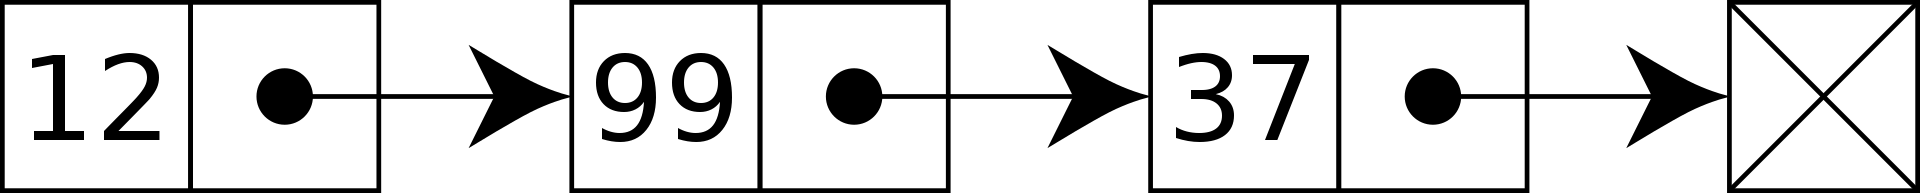
\includegraphics[width=\textwidth]{list.png}
\caption{Příklad lineárního seznamu o třech položkách s číselnými daty}
\end{figure}
\begin{figure}[h]
\centering
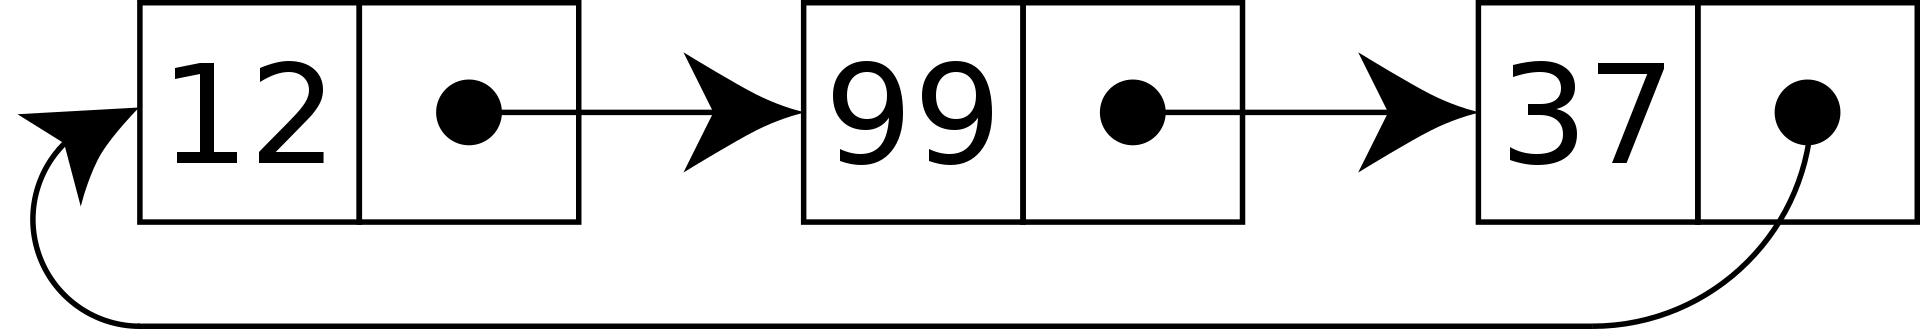
\includegraphics[width=\textwidth]{circular.png}
\caption{Příklad cyklického lineárního seznamu}
\end{figure}
\end{frame}

\section{Výhody a nevýhody}
\begin{frame}
\frametitle{Výhody a nevýhody}
Lineární seznam se často přirovnává a je použitím podobný k poli, proto se nabízí tyto datové struktury porovnat.
\pause

\begin{itemize}
    \item Výhody:
    \begin{itemize}
        \item Je to dynamická struktura a lze snadno měnit počet nebo pořadí položek
        \item Přidání či odebrání ze seznamu má konstantní časovou náročnost $O(1)$
        \item Seznam může být i cyklický (poslední položka ukazuje zpět na první) nebo oboustranně vázaný
    \end{itemize}
    \pause
    \item Nevýhody:
    \begin{itemize}
        \item Přístup do seznamu má lineární časovou složitost $O(n)$
        \item Není možný náhodný přístup
        \item Oproti poli zabere více paměti
    \end{itemize}
\end{itemize}
\end{frame} 

\section{Operace s lineárním seznamem}
\subsection{Inicializace seznamu}
\begin{frame}[fragile]
\frametitle{Inicializace seznamu}
Struktura položky:
\begin{minted}[frame=single]{c}
typedef struct node{
    int data;
    node *next;
} node;
\end{minted}
\bigskip

Inicializace seznamu:
\begin{minted}[frame=single]{c}
node *first = NULL;
\end{minted}
\end{frame}

\subsection{Zjištění délky seznamu}
\begin{frame}[fragile]
\frametitle{Zjištění délky seznamu}
\begin{minted}[frame=single]{c}
int len(node *first){
    int i;
    node *item = first;
    for(item->next != NULL){
        item = item->next;
        i++;
    }
    
    return i;
}
\end{minted}
\end{frame}

\subsection{Přidání položky do seznamu}
\begin{frame}[fragile]
\frametitle{Přidání položky do seznamu}
\begin{minted}[frame=single]{c}
void addItem(struct node *first, node *new, int pos){
    node *item = first;
    for(int i = 0; i < pos; i++){
        item = item->next;
    }
    
    new->next = item->next;
    item->next = new;
}
\end{minted}
\end{frame}

\subsection{Odebrání položky ze seznamu}
\begin{frame}[fragile]
\frametitle{Odebrání položky ze seznamu}
\begin{minted}[frame=single]{c}
void removeItem(node *first, int pos){
    node *item = first, *previous;
    for(int i = 0; i < pos; i++){
        previous = item;
        item = item->next;
    }
    
    previous->next = item->next;
}
\end{minted}
\end{frame}

\section{Zdroje}
\begin{frame}
\frametitle{Zdroje}
\begin{itemize}
    \item \url{https://en.wikipedia.org/wiki/Linked_list}
    \item \url{https://people.engr.ncsu.edu/efg/210/s99/Notes/LinkedList.1.html}
    \item \url{http://cslibrary.stanford.edu/103/LinkedListBasics.pdf}
\end{itemize}
\end{frame}
\end{document}